\section{Test mit modulspezifischen Klauseln} % 47 - 41
\label{sec:test_modul}

Dieser Test bezieht zusätzlich zu den Basisklauseln die Klauseln aus Tabelle \ref{fig:additional_clauses_mod} mit ein.
Ausgenommen sind davon jedoch die zusätzlichen Klauseln für den Addierer, die in Abschnitt \ref{sec:test_234} separat getestet werden.
Die Ergebnisse sind in Abbildung \ref{fig:data_modul} dargestellt.
Insgesamt reduziert sich die Testlaufzeit um mehr als 50\% wobei die XOR-Variante nach wie vor schneller ist.
Ein weiterer Vorteil der XOR-Variante in diesem Test ist die Anzahl der unterschiedlichen Ergebnisse. Durch die zusätzlichen
Klauseln konnte CryptoMiniSat mehr Berechnungen durchführen und es vermeiden Belegungen zu raten.
\begin{figure}[!h]
  \centering
  \begin{minipage}[c]{0.45\textwidth}
  \begin{flushleft}Gesamtdauer ohne XOR: 91:28:43\end{flushleft}
  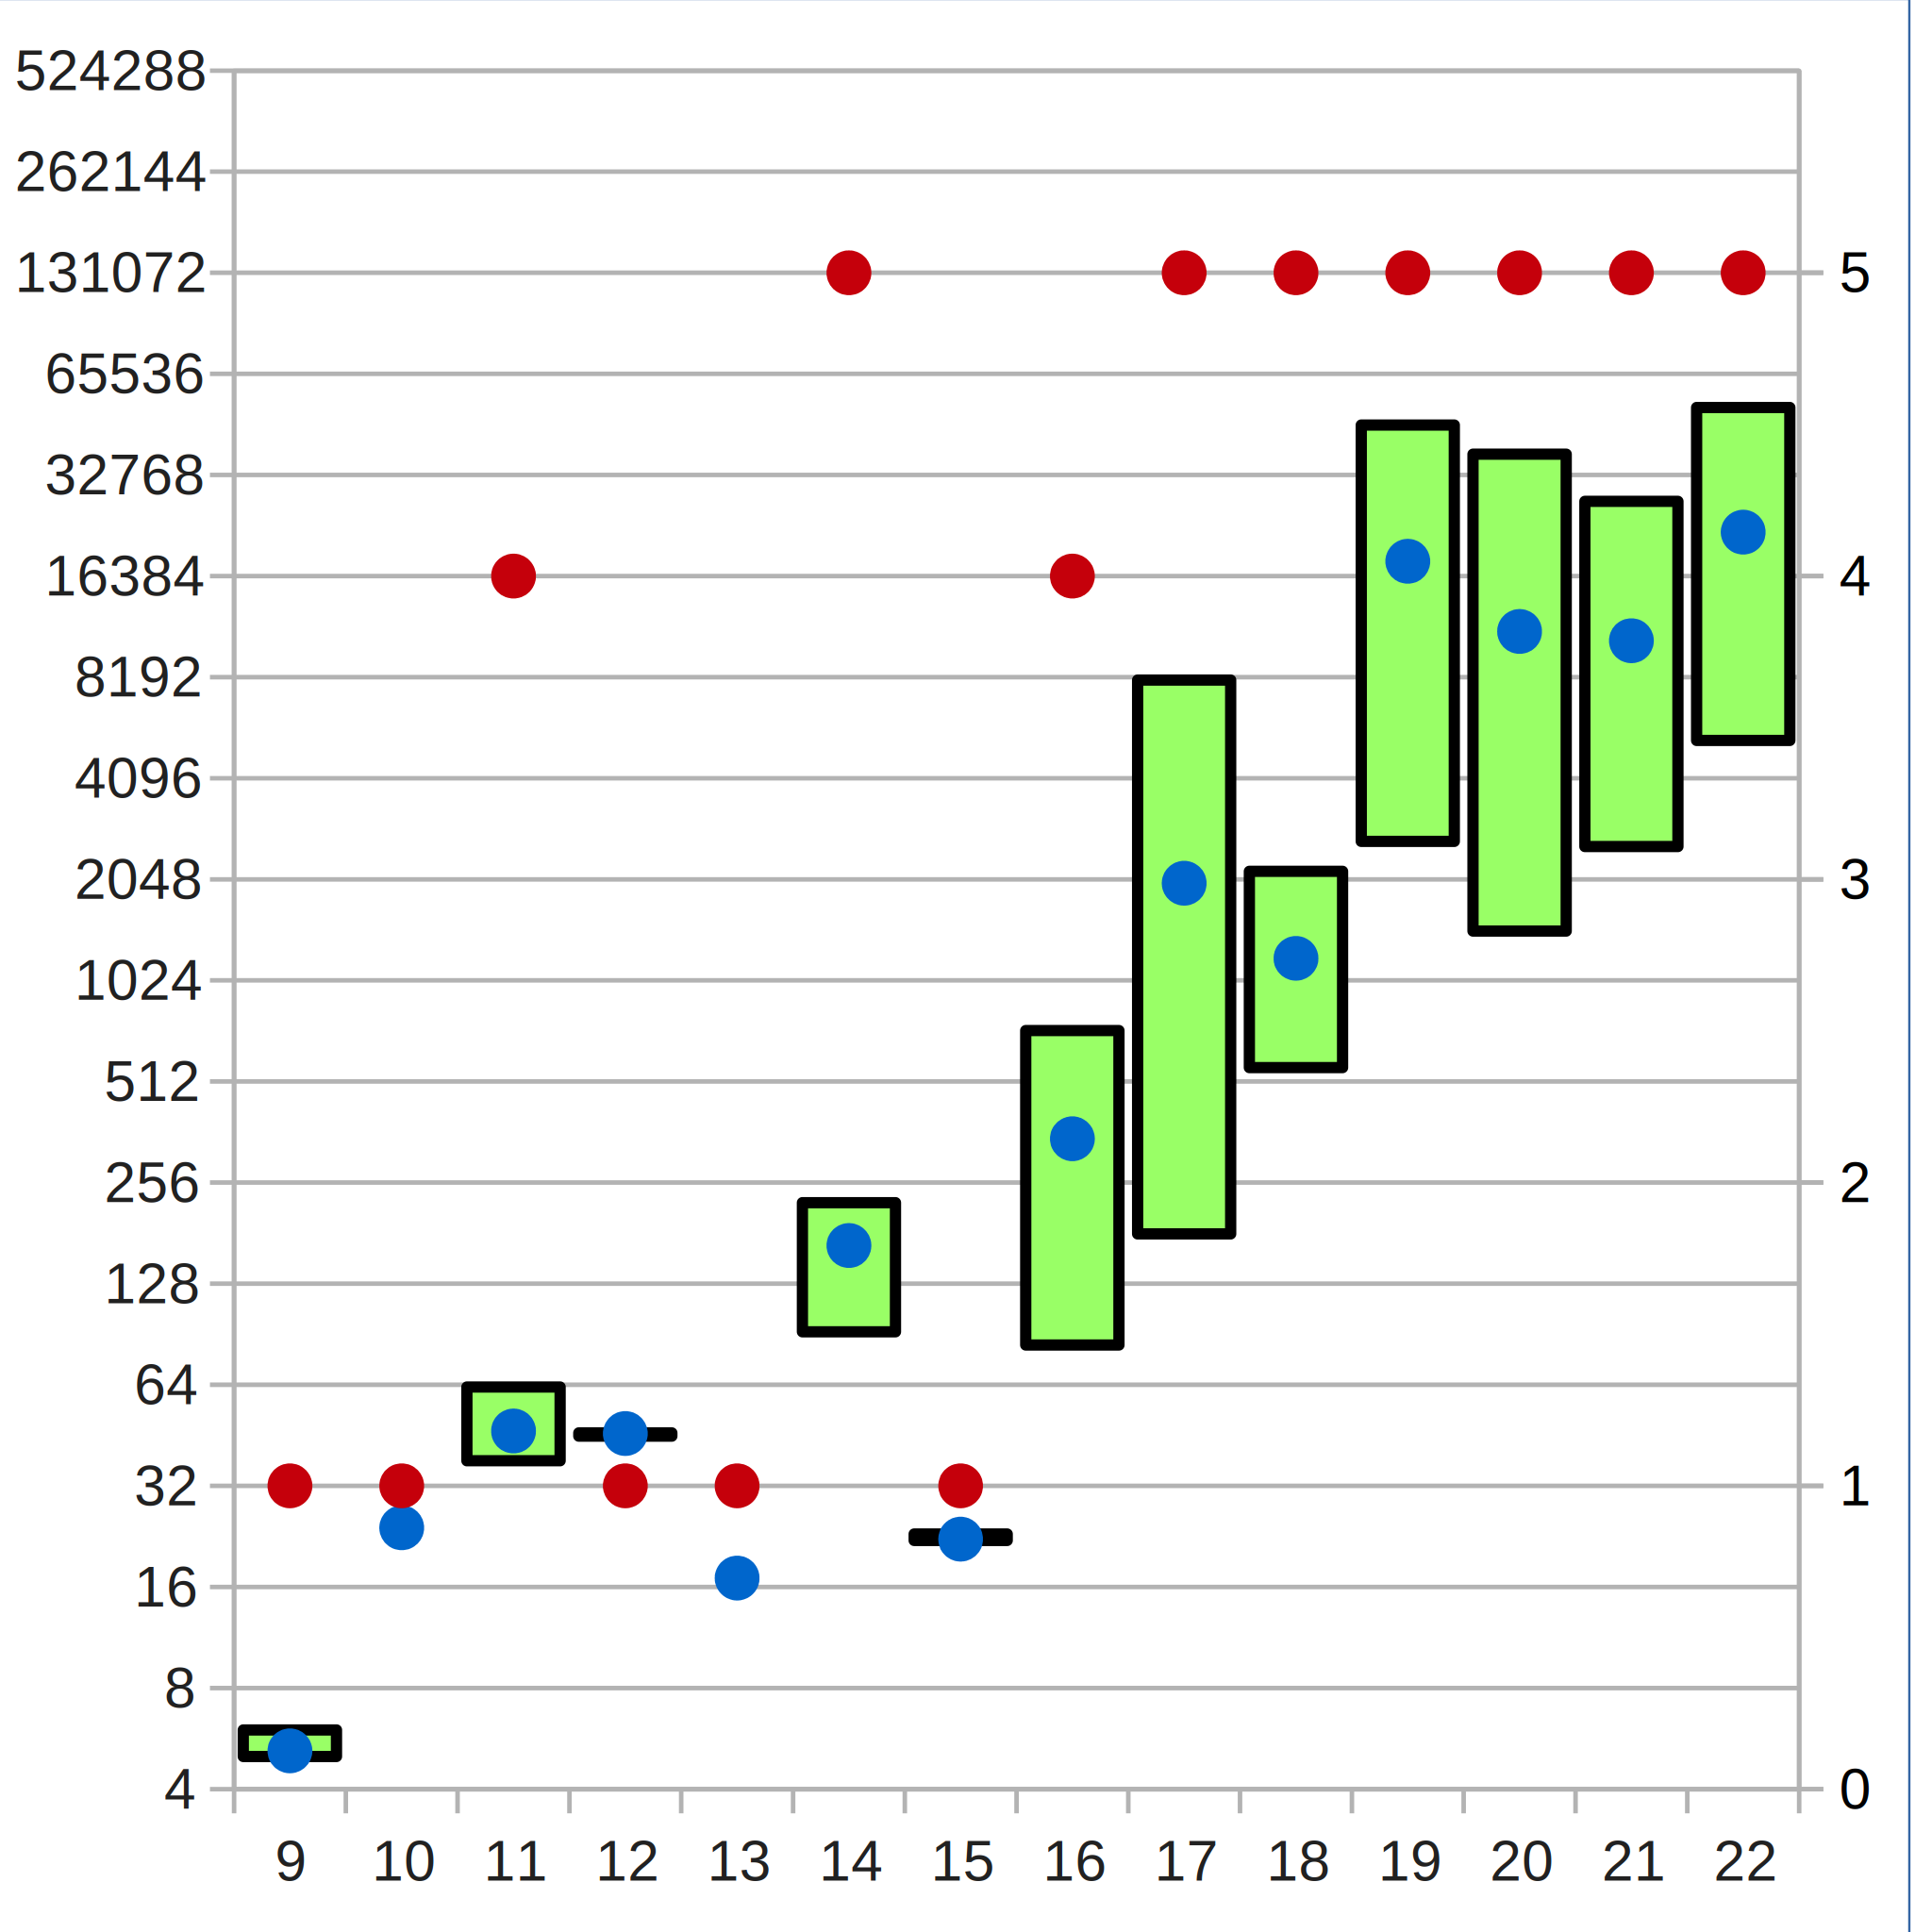
\includegraphics[scale=0.55]{images/data_modul_knf}
  \end{minipage}
  \begin{minipage}[c]{0.09\textwidth}
  ~~
  \end{minipage}
  \begin{minipage}[c]{0.45\textwidth}
  \begin{flushleft}Gesamtdauer mit XOR: 69:07:57\end{flushleft}
  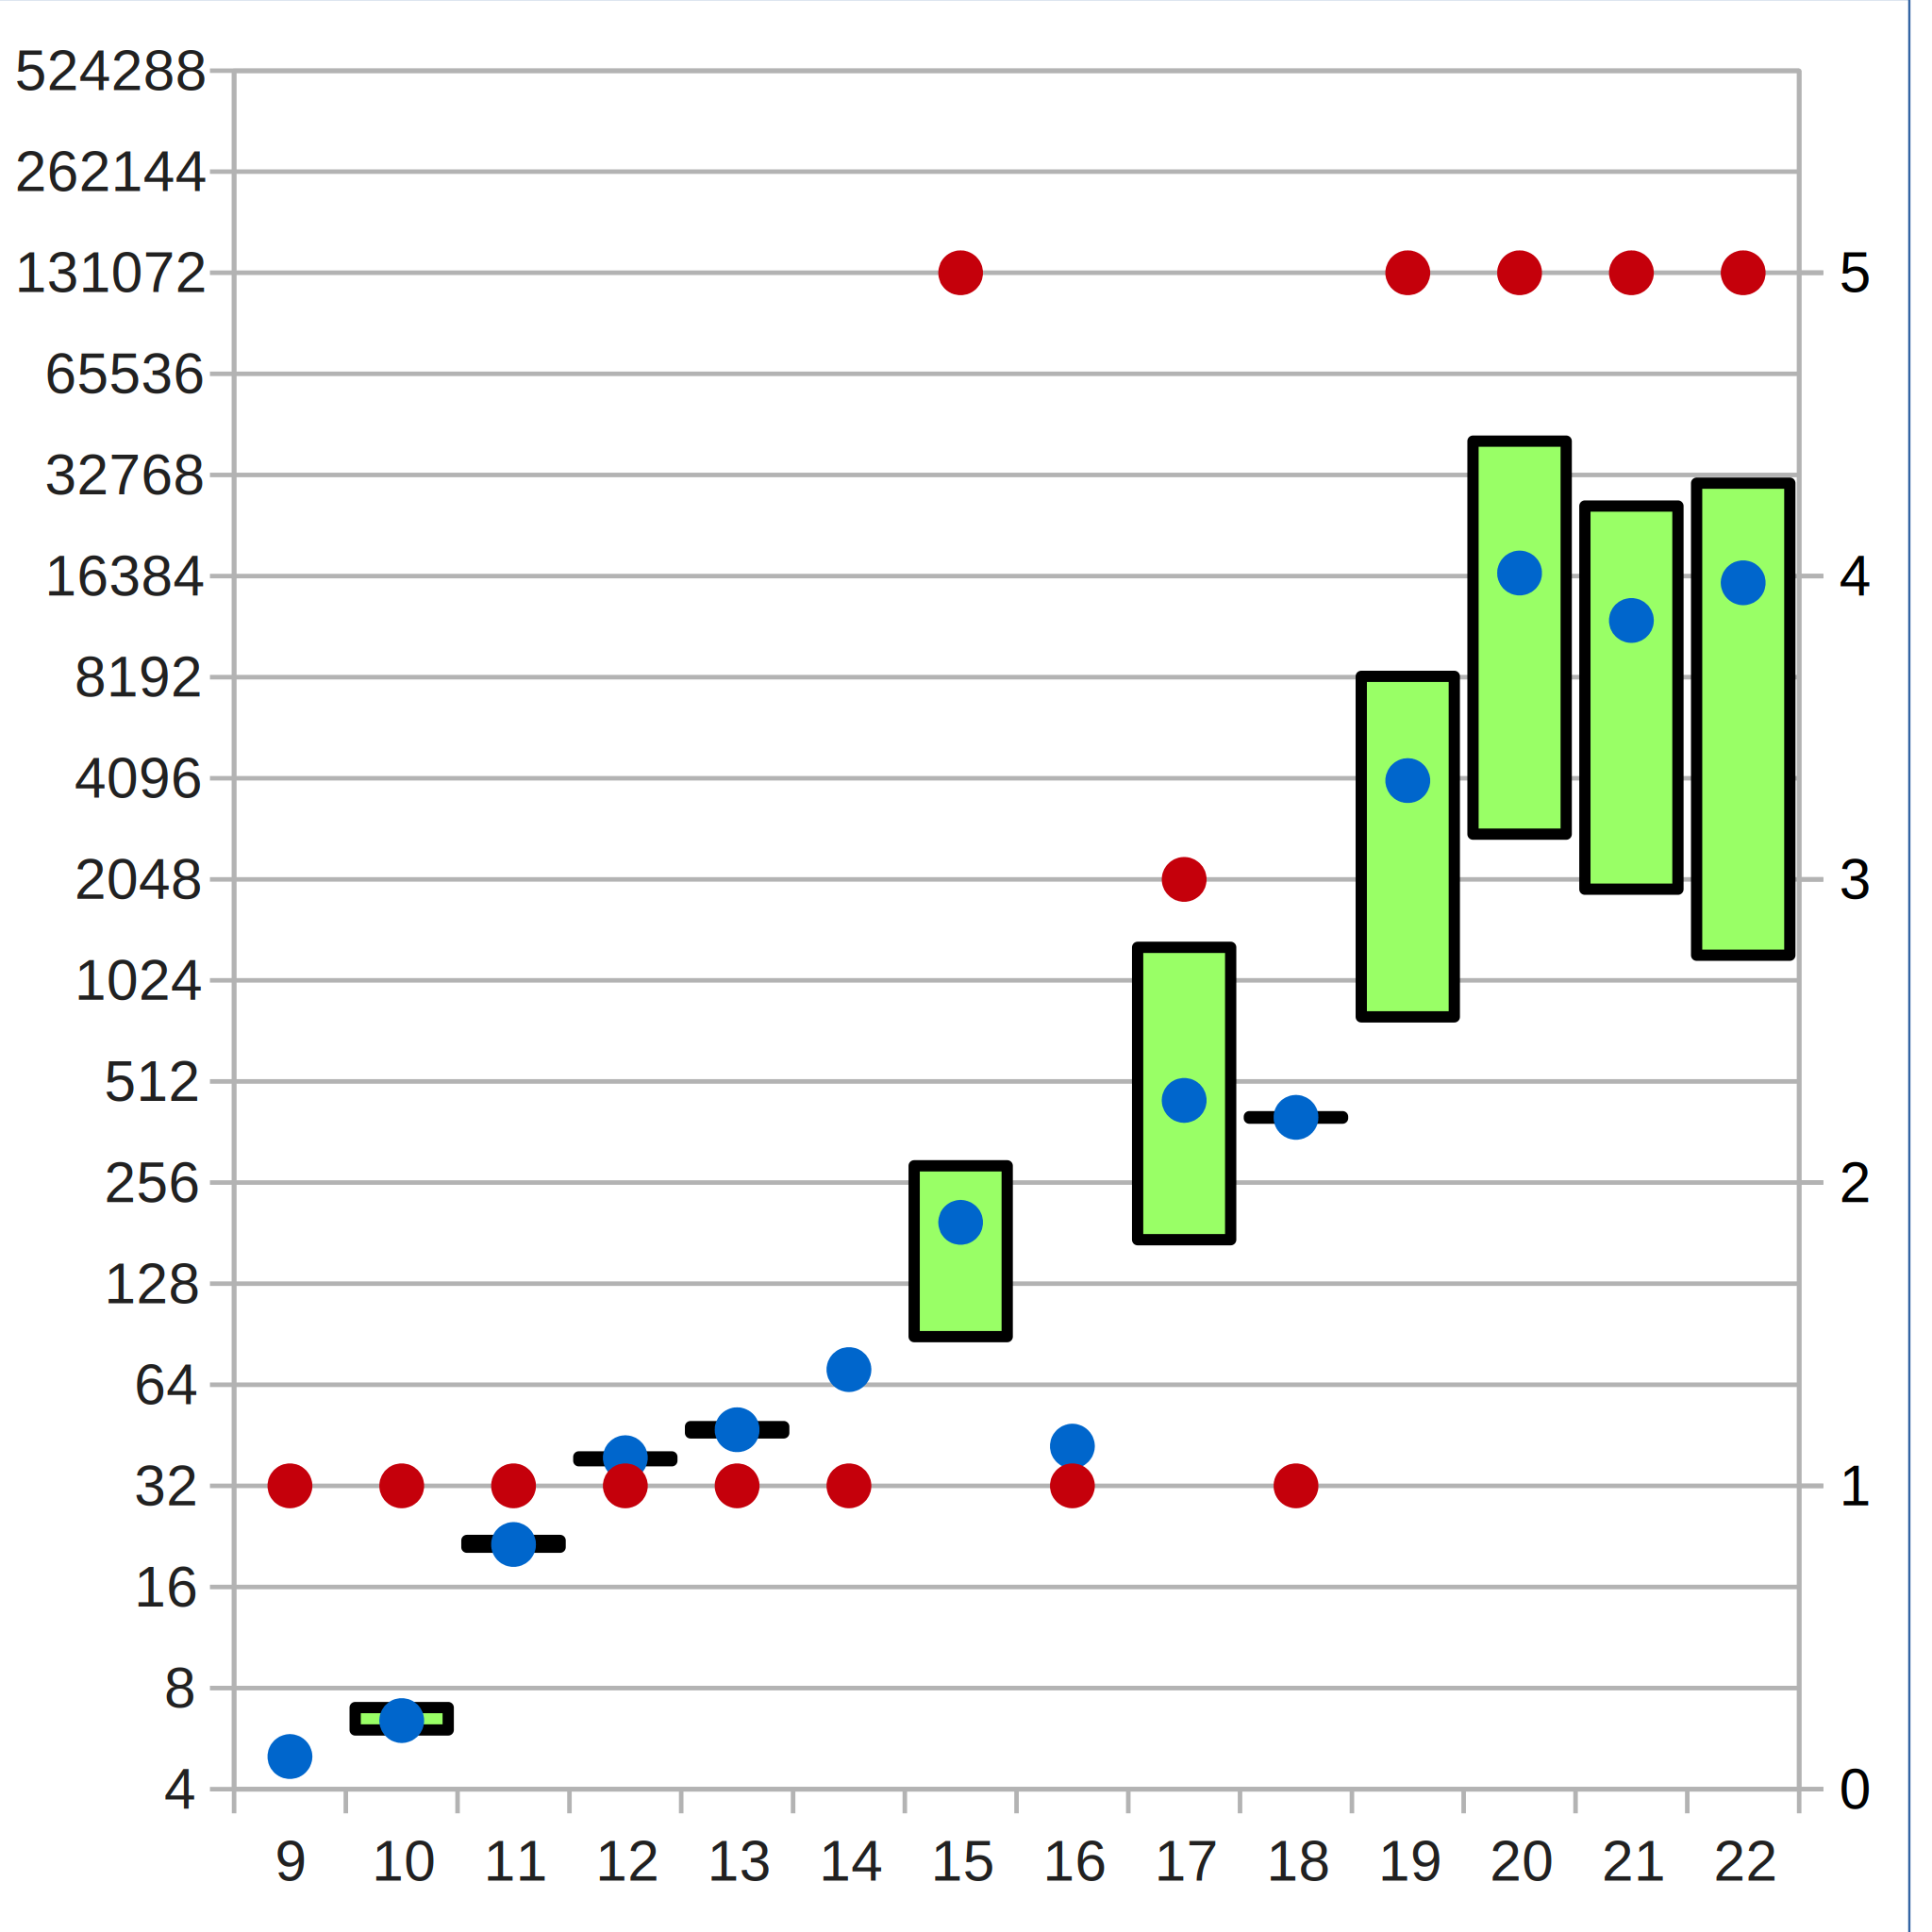
\includegraphics[scale=0.55]{images/data_modul_xor}
  \end{minipage}
  \caption{Ergebnisse mit modulspezifischen Klauseln}
  \label{fig:data_modul}
\end{figure}